
%%%%%%%%%%%%%%%%%%%%%%%%%%%%%%%%%%%%%%%%%%%%%%%%%%%%%%%%%%%%%%%%%%%%%%%
%                            Introduction                             %
%%%%%%%%%%%%%%%%%%%%%%%%%%%%%%%%%%%%%%%%%%%%%%%%%%%%%%%%%%%%%%%%%%%%%%%


\chapter*{Introduction}
\addcontentsline{toc}{chapter}{Introduction}
\label{cha:introduction}
\markboth{Introduction}{Introduction}
%\setcounter{chapter}{-1}
%\chapter{Introduction}
%%\addcontentsline{toc}{chapter}{Introduction}
%\label{cha:introduction}

\graphicspath{{Chapter0-Introduction/Figs/Vector/}{Chapter0-Introduction/Figs/}}

The ultimate goal of robotics is to make robots realize some tasks to assist humans in their various fields of work.
The tasks, as well as the robots used to fulfill them, are various.
For example, it can be a robotic arm building a car in a factory, a surgeon robot operating on a human body, a submarine robot exploring the wreckage of a ship, or a humanoid robot exploring and fixing a destroyed plant.

\begin{figure}[ht]
  \centering
  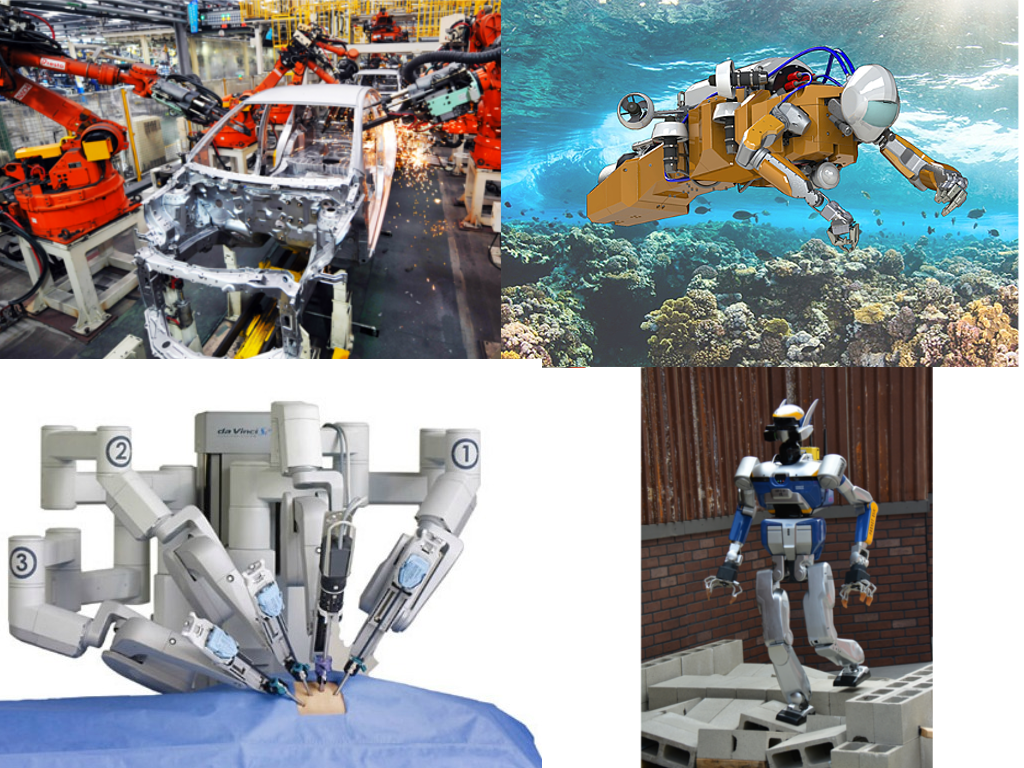
\includegraphics[width=0.9\textwidth]{various-tasks.png}
\label{fig:various}
\end{figure}

The DARPA Robotics Challenge has shone some light on the capabilities and limitations of humanoid robots.
This competition brought together robotics groups from Universities, laboratories, and private companies to work on a common goal: develop a partially teleoperated robot system that can succeed in several tasks without any human physical intervention.
The robots were required to drive a car, open a door, climb stairs, cross debris, drill a hole in a wall, etc.
All these tasks can usually be broken down into sets of elementary tasks in human language, such as `put hand in contact with target', `put foot on next step', `avoid collision with that object', `maintain stability' or `look in that direction'.
As is, these tasks do not mean anything for the robot that has no knowledge of its interaction with the world, or of human language.
The way to complete a task must be provided to the robot as a sequence of joint configurations.

Tasks are generally expressed in the operational space of the robot, and to satisfy them, one needs to find a configuration of the robot, in its articular space, that allows completion of the task, and also to find a way for the robot to reach that configuration.
For mobile underactuated robots, such as humanoids, the position of its base depends on the configuration of the joints as well as on the locations of the contacts that the robot makes with the environment.
Thus, even if each link of the robot is actuated, it is possible that for a given set of contacts, some tasks are out of reach, in which case, it becomes necessary to modify the set by adding or removing some contacts.
Much like humans, the robot must choose appropriate parts of its body to create contacts with the surrounding environment in order to support its motion while avoiding obstacles and reaching its goal.
A whole motion can be described by a sequence of contact creations and releases with joint trajectories inbetween successive elements of the sequence.

Computing a trajectory to follow, and actually following it, are respectively handled by the trajectory generator and controller of the robot.
Trajectory generation and control are by themselves complete sub-fields in robotics, and they both often rely on being given some key postures to help guide the robot's motion(e.g. initial, intermediate and final configurations).

Computing a sequence of key configurations that allows the robot to complete some tasks is handled by the contact planner, which explores the space of possible sets of contacts between the robot and its environment in order to devise a path, composed of `viable' configurations, along which contacts are iteratively added and removed, that leads to the task completion.
A configuration is deemed `viable' if it guarantees the integrity of the robotic system by respecting its intrinsic limitations, avoiding undesired collisions and guaranteeing its stability.
Depending on the complexity of the scenario, different approaches to planning can be used.
On flat terrains, the robot can walk based on a cyclic motion and the locations of footsteps can be generated by a footstep planner using some simplified models to maintain its stability.
As the environment becomes more difficult to cross, in cumbersome and unstructured environments for example, hands may come into play together with feet to help with the motion.
Narrow passages may even require other parts of the body (knees, elbows, back\dots) to make contact in order to support the motion.
In such multi-contact scenarios, less simplifications are possible, and the problem of finding a `viable' configuration is traditionally formulated as a collection of constraints and objective function in the operational and articular spaces of the robot, that translate the tasks to achieve, as well as the conditions for the configuration to be viable.
Once a satisfactory configuration is found, it is a candidate to be added to the planner's path.
%Such problems, that we call multi-contact posture generation problems, usually do not have closed-form solutions, and are solved as optimization programs using off-the-shelf optimization solver.

The formulation and resolution of multi-contact posture generation problems, as the one described above, are the missions of the `Posture Generator' (PG) and the development of this tool is the central topic of this dissertation.
Computing robot configurations to meet the requirements of a given set of tasks, within a viable state, is a recurrent problem whose complexity grows with that of the robot.
When the robotic problem studied becomes too complex for closed-form solutions, it is formulated as a nonlinear optimization program and solved using optimization algorithms.
The PG is a key tool for many robotics applications and as such, it is an important component of any robotics framework.
It needs to be efficient at finding a solution when one exists, and at figuring out if a problem is not feasible.
The speed of generating a multi-contact sequence is directly related to the quality of the PG, which is directly related to the quality of the optimization algorithm that it uses.

The formulation of a posture generation problem is often a cumbersome and time-consuming task for the programmer, requiring a fine-tuning of the problem's constraints and cost functions, as well as of the solver, to get satisfactory results.
In this thesis, we present a posture generation framework that makes the development of posture generation problems easier, as will as richer, by proposing several extensions to their formulation.

%Planning a sequence of key configurations is a necessary step in devising a robot motion.
%Once the key stances of the motion have been identified by the contact planner, they can be used by the controller or the trajectory planner and finally the motion can be achieved by the robot.

%All the aforementioned planning methods rely on the fact that we have a tool to decide if a proposed set of contacts is feasible or not for a given robot.
%The tool used for finding a robot configuration that satisfies a set of constraints, like the geometric constraints of contact or the stability of the robot, is called a `Posture Generator' (PG) and the development of this tool is the main topic of this dissertation.

%The mission of a posture generator, for a polyarticulated system, is to find a configuration in which the system satisfies a set of constraints while minimizing a defined criterion.
%Closed-form solutions may be possible for relatively simple systems and tasks, like a 6 DoF robotic arm that is required to reach a point with its end effector.
%However, computing robot configurations to meet the requirements of a given set of tasks, within a viable state, is a recurrent problem whose complexity grows with that of the robot.
%When the robotic problem studied becomes too complex for closed-form solutions, it is formulated as a nonlinear optimization program and solved using optimization algorithms.
%The PG is a key tool for many robotics applications and as such, it is an important component of any robotics framework.
%It needs to be efficient at finding a solution when one exists, and at figuring out if a problem is not feasible.
%The speed of generating a multi-contact sequence is directly related to the quality of the PG, which is directly related to the quality of the optimization algorithm that it uses.

Once the problem of posture generation is formulated, its resolution can take place.
The variables of a robotics problem sometimes naturally belong to a non-Euclidean manifold $\mathcal{M}$, like $SO(3)$ for the 3D rotation of the base of a mobile robot.
A manifold is a topological space that locally resembles a Euclidean space near each point.
Each point of an n-dimensional manifold has a neighborhood that is homeomorphic to the Euclidean space of dimension n.
An n-dimensional non-Euclidean manifold cannot always be globally parameterized over a subset of $\mathbb{R}^n$ without presenting problems of singularity.
Most of the optimization solvers available make the assumption that the search space is Euclidean, and thus, do not feature the capability of solving problems on non-Euclidean manifolds natively.
But it is often possible to parametrize $\mathcal{M}$ over a Euclidean space of higher dimension with added constraints (e.g. unit quaternions, rotation matrices).
It is then possible to solve those problems with classical solvers at the cost of additional variables, constraints and special treatments in the resolution of the optimization problem.
There exists some methods and algorithms to solve optimization problems on non-Euclidean manifolds with no substantial extra cost and guaranteeing a good coverage of the manifolds without facing parameterization singularities, and with the minimal number of parameters.
However, to our knowledge, these are focused on addressing non-constrained optimization.

%Usually, the solver used for solving optimization problems is a black box on which the user has a very limited control.
Through this thesis, we develop our own nonlinear constrained optimization solver on manifolds and use it to solve optimization problems on their native search manifolds. We will exhibit the interests of such resolution methods for posture generation problems as well as a few other types of problems.
This has the advantage that, unlike off-the-shelf solvers which are often a black box on which the user has very limited control, we have full control over that solver and can specialize/modify it to fit our needs.

%Satisfying a task requires that the joints of the robot reach a configuration for which the task is completed.
%A robot is made of a collection of bodies (or links) that are linked together by joints actuated by motors.
%A robot's configuration consists of the position and orientation of its base body, and the configuration of each of its joints.
%This problem can be divided in two sub-problems:
%\begin{itemize}
  %\item Finding configurations to satisfy the tasks
  %\item Reaching those configurations with the robot
%\end{itemize}
%Thus, the action of satisfying a task comes down to moving from an initial configuration to a goal configuration.

%Finding the configurations to satisfy the tasks is the problem that we call Posture Generation(PG).

%Traditionally, the constraints and objective functions that compose the posture generation problem are written in the robot's operational and articular space to compute an optimization problem that is in turn solved by a nonlinear optimization algorithm.
%The formulation of such problem is usually a cumbersome and time-consuming task due to the limited

%Depending on the complexity of the Posture Generation problem, different methods of formulation and resolution can be used.

%Robots can be divided into two broad categories: fixed-base robots and mobile robots.
%As the name suggests, the first type of robots have fixed bases, their workspace is predefined by their geometry, and they are usually fully actuated.
%This means that the robot has as many degrees of freedom (DoF) as it has actuators. Thus, any particular joint configuration leads to a unique robot posture.
%On the contrary, mobile robots are always underactuated such that the robot has more DoF than actuators.
%Each link of the robot is actuated, but the position of the base of the robot depends on the configuration of the joints as well as on the locations of the contacts that the robot makes with the environment.

%Humanoid robots are expected to move and achieve tasks in ways similar to humans.
%On flat surfaces, they can walk based on a cyclic motion and the locations of footsteps can be generated by a footstep planner using some simplified models to maintain the robot's stability.
%In cumbersome and unstructured environments, we humans move in a non-gaited acyclic way: we choose appropriate parts of our body to create contacts with the surrounding environment in order to support the motion of the remaining parts while avoiding obstacles.
%A whole motion is a sequence of contact creations and releases.

%Since we are biped, we mostly use our feet to move.
%As the environment becomes more difficult to cross, hands may come into play together with feet to help with the motion.
%Narrow passages may even require other parts of our body (knees, elbows, back\dots) to make contact in order to support the motion.

%\paragraph{Specificities of our approach}
%If we consider a problem of posture generation on a mobile robot with $n$ joints, the configuration space of the joints of the robot is $\mathbb{R}^n$ and the configuration space of the position and orientation of its base body is $SE(3) = \mathbb{R}^3\times SO(3)$.
%Thus, the variable that describes the configuration of the robot in the optimization problem lives in $\mathbb{R}^3\times SO(3) \times \mathbb{R}^n$.
%$SO(3)$ is by nature a non-Euclidean manifold, it cannot be parameterized on an open subset of Euclidean space without having to deal with problems of gimbal lock.
%The gimbal lock is a singularity that happens when parameterizing $SO(3)$ on $\mathbb{R}^3$, with Euler angles, for example, and when two axis of rotation become aligned, in that situation, 2 elements of the parameterization correspond to the same rotation.
%Thus, one degree of freedom is lost.
%Note that this singularity can block the optimization algorithm and that it is only due to the choice of parameterization, it is not intrinsic to the manifold $SO(3)$.
%It is possible to parameterize $SO(3)$ without having to face singularities by parameterizing it over another non-Euclidean manifold.
%The most common ones are the unit quaternion space and the $3\times 3$ rotation matrix.
%Most of the solvers available make the assumption that the search space is Euclidean, which makes is complicated to use quaternion or rotation matrix efficiently.
%To put it simply, for the unit quaternion parameterization, a variable on $SO(3)$ is represented by 4 parameters, the coefficients of the quaternion and an equality constraint needs to be added to the optimization problem to ensure that the quaternion is of norm 1, $\{q\in\mathbb{R}^4:||q||=1\}$.
%Similarly, if a variable is parameterized by a rotation matrix, then the variable $M$ has 9 parameters and several constraints need to be added to the problem so that M is symmetric, positive definite and its determinant is 1 $\{M\in\mathbb{R}^{3\times 3}:M^T M = \mathbb{I}_3\  \&\ \det (M) = 1\}$.
%Similar issues can be found with the parameterization of other non-Euclidean manifold, like $S^2$ for example.

%There exists some methods and algorithms to solve optimization problems on non-Euclidean manifolds with no substantial extra cost and guaranteeing a good coverage of the manifolds without facing parameterization singularities and with the minimal number of parameters, though to our knowledge, they are focused on non-constrained optimization.

\paragraph{Contributions and plan}
The main focuses of this thesis are the formulation and the resolution of problems of posture generation for robotics systems using nonlinear optimization on manifolds.
Our contribution is two fold, on one hand we propose extensions and improvements on the ways to formulate a posture generation problem, and on the other hand, we investigate new ways of solving these problems.
The organization of this thesis is as follows:
%In Chapters~\ref{cha:state_of_the_art} and~\ref{cha:posture_generation_problem_formulation}, we present the background of posture generation, with respectively a state of the art and a presentation of the detailed formulation of a posture generation problem.
%We present several
\begin{itemize}
  \item In Chapter~\ref{cha:state_of_the_art_and_problem_definition} we describe the state of the art of posture generation and optimization on manifolds.
  \item In Chapter~\ref{cha:posture_generation_problem_formulation}, we present the detailed formulation of a posture generation problem.
  \item In Chapter~\ref{cha:extensions_of_posture_generation} we present three different and unrelated contributions: two formulation extensions, one allowing to generate non-inclusive contacts between convex surfaces, the other is the exact derivation of the torques in the actuators of a robot.
  We then present our endeavor to use the `Lifted Newton Method' to solve posture generation problems.
  \item Chapter~\ref{chapter:optimization_on_noneuclidean_manifolds} describes the principles of nonlinear optimization over non-Euclidean manifolds and our implementation of a solver based on those principles.
  \item In Chapter~\ref{ch:PG}, we present a framework that simplifies and extends the formulation of posture generation problems by formulating and solving the optimization problem over native non-Euclidean manifolds, managing automatically the variables of the problems, and proposing a framework that formalizes and simplifies the writing of functions on geometric entities often used in robotics.
  \item In Chapter~\ref{cha:evaluation_and_experimentation}, we evaluate the performances of our solver on manifolds, and the performances of our posture generator. We then present preliminary work on the generation of postures on a sensor acquired environment.
\end{itemize}


